%
% File acl2018.tex
%
%% Based on the style files for ACL-2017, with some changes, which were, in turn,
%% Based on the style files for ACL-2015, with some improvements
%%  taken from the NAACL-2016 style
%% Based on the style files for ACL-2014, which were, in turn,
%% based on ACL-2013, ACL-2012, ACL-2011, ACL-2010, ACL-IJCNLP-2009,
%% EACL-2009, IJCNLP-2008...
%% Based on the style files for EACL 2006 by 
%%e.agirre@ehu.es or Sergi.Balari@uab.es
%% and that of ACL 08 by Joakim Nivre and Noah Smith

\documentclass[11pt,a4paper]{article}
\usepackage[hyperref]{acl2018}
\usepackage{times}
\usepackage{latexsym}
\usepackage{amsmath}
\usepackage{url}

\usepackage{tabularx}

\usepackage{titlesec}
\setcounter{secnumdepth}{3}

\usepackage{graphicx}
\graphicspath{ {graphics/} }

\usepackage[inline]{enumitem}

\aclfinalcopy % Uncomment this line for the final submission
%\def\aclpaperid{***} %  Enter the acl Paper ID here

%\setlength\titlebox{5cm}
% You can expand the titlebox if you need extra space
% to show all the authors. Please do not make the titlebox
% smaller than 5cm (the original size); we will check this
% in the camera-ready version and ask you to change it back.

\newcommand\BibTeX{B{\sc ib}\TeX}


%%%
%% Variables

\newcommand{\mntestsamples}{1120 }
\newcommand{\mntrainsamples}{3374 }

\newcommand{\mnintentlabels}{67}
\newcommand{\mnentitylabels}{24}
%%%

\title{Movie Domain Bot \\ Final project}

\author{Andrea Tupini \\
  MAT.  194578 \\
  {\tt andrea.tupini@studenti.unitn.it}}

\date{}

\begin{document}
	
\maketitle

\begin{abstract}
	
	This project consisted of building a bot that could answer questions on the movie domain. We had to build both the NLU and dialogue modules. In this report, we'll see a bit about how the bot works and the decision made during its design, plus some encountered problems.
	
\end{abstract} 

\section{Introduction}
	
	This is the report for the final project of the \textit{Language Understanding System Course} \cite{lus-website} at University of Trento year  2017/2018. 
	
	The bot was built using the Rasa stack (a combination of rasa NLU  and rasa\_core) and it was trained on data provided for this project about the movie domain. We'll analyze a bit the data, define the NLU and dialogue modules and their respective components, and finally evaluate the performance of the NLU module and present some difficulties found during development and design of the bot.

	
\section{Data Analysis}
\label{sec-data-analysis}
	
	The original data that was provided consisted mainly of two things: a movie database that contains various information on the movie domain, and the data needed for training the NLU module of the bot (this was given in NLSPARQL format).
	
	\subsection{NLU Data}
	\label{ssec-nlu-data}
	
		Originally, the provided NLU data consisted of the following files: 
		
		\begin{description}
			\item[NLSPARQL.test] words and IOB tags for testing (contains \mntestsamples examples)
			\item[NLSPARQL.train] words and IOB tags for training (contains \mntrainsamples examples)
			\item[NLSPARQL.test.utt.labels] contains labels on what each question in the test set is about              
			\item[NLSPARQL.train.utt.labels] labels of questions in training set
		\end{description}
	
		Both the test and train sets are composed of sentences examples in which \textit{entities} are annotated using the IOB notation, and each sentence is also labeled with an \textit{intent}. Both entities and intents are defined more in-depth in section \ref{ssec-nlu-module}.
	
		The provided format is not recognized by Rasa, so these had to be converted to a properly formatted \textit{json} file. In the rasa format, for each sentence, we need to provide which are the entities and intent of the sentence. Extracting entities was just a simple matter of using the IOB tags that are not \textit{O}s, and the intents were taken directly from the \textit{labels} files. In the dataset there are \textbf{\mnentitylabels} different entity labels and \textbf{\mnintentlabels} intent labels. Note that the original dataset was modified a bit: very similar entities and intents were merged.
		
		Here we have a graphic that shows the count of different entity types provided in the dataset (note that it is log scaled so as to account for the difference between the most common entity and the least common one):
		
		\hspace*{-0.4cm}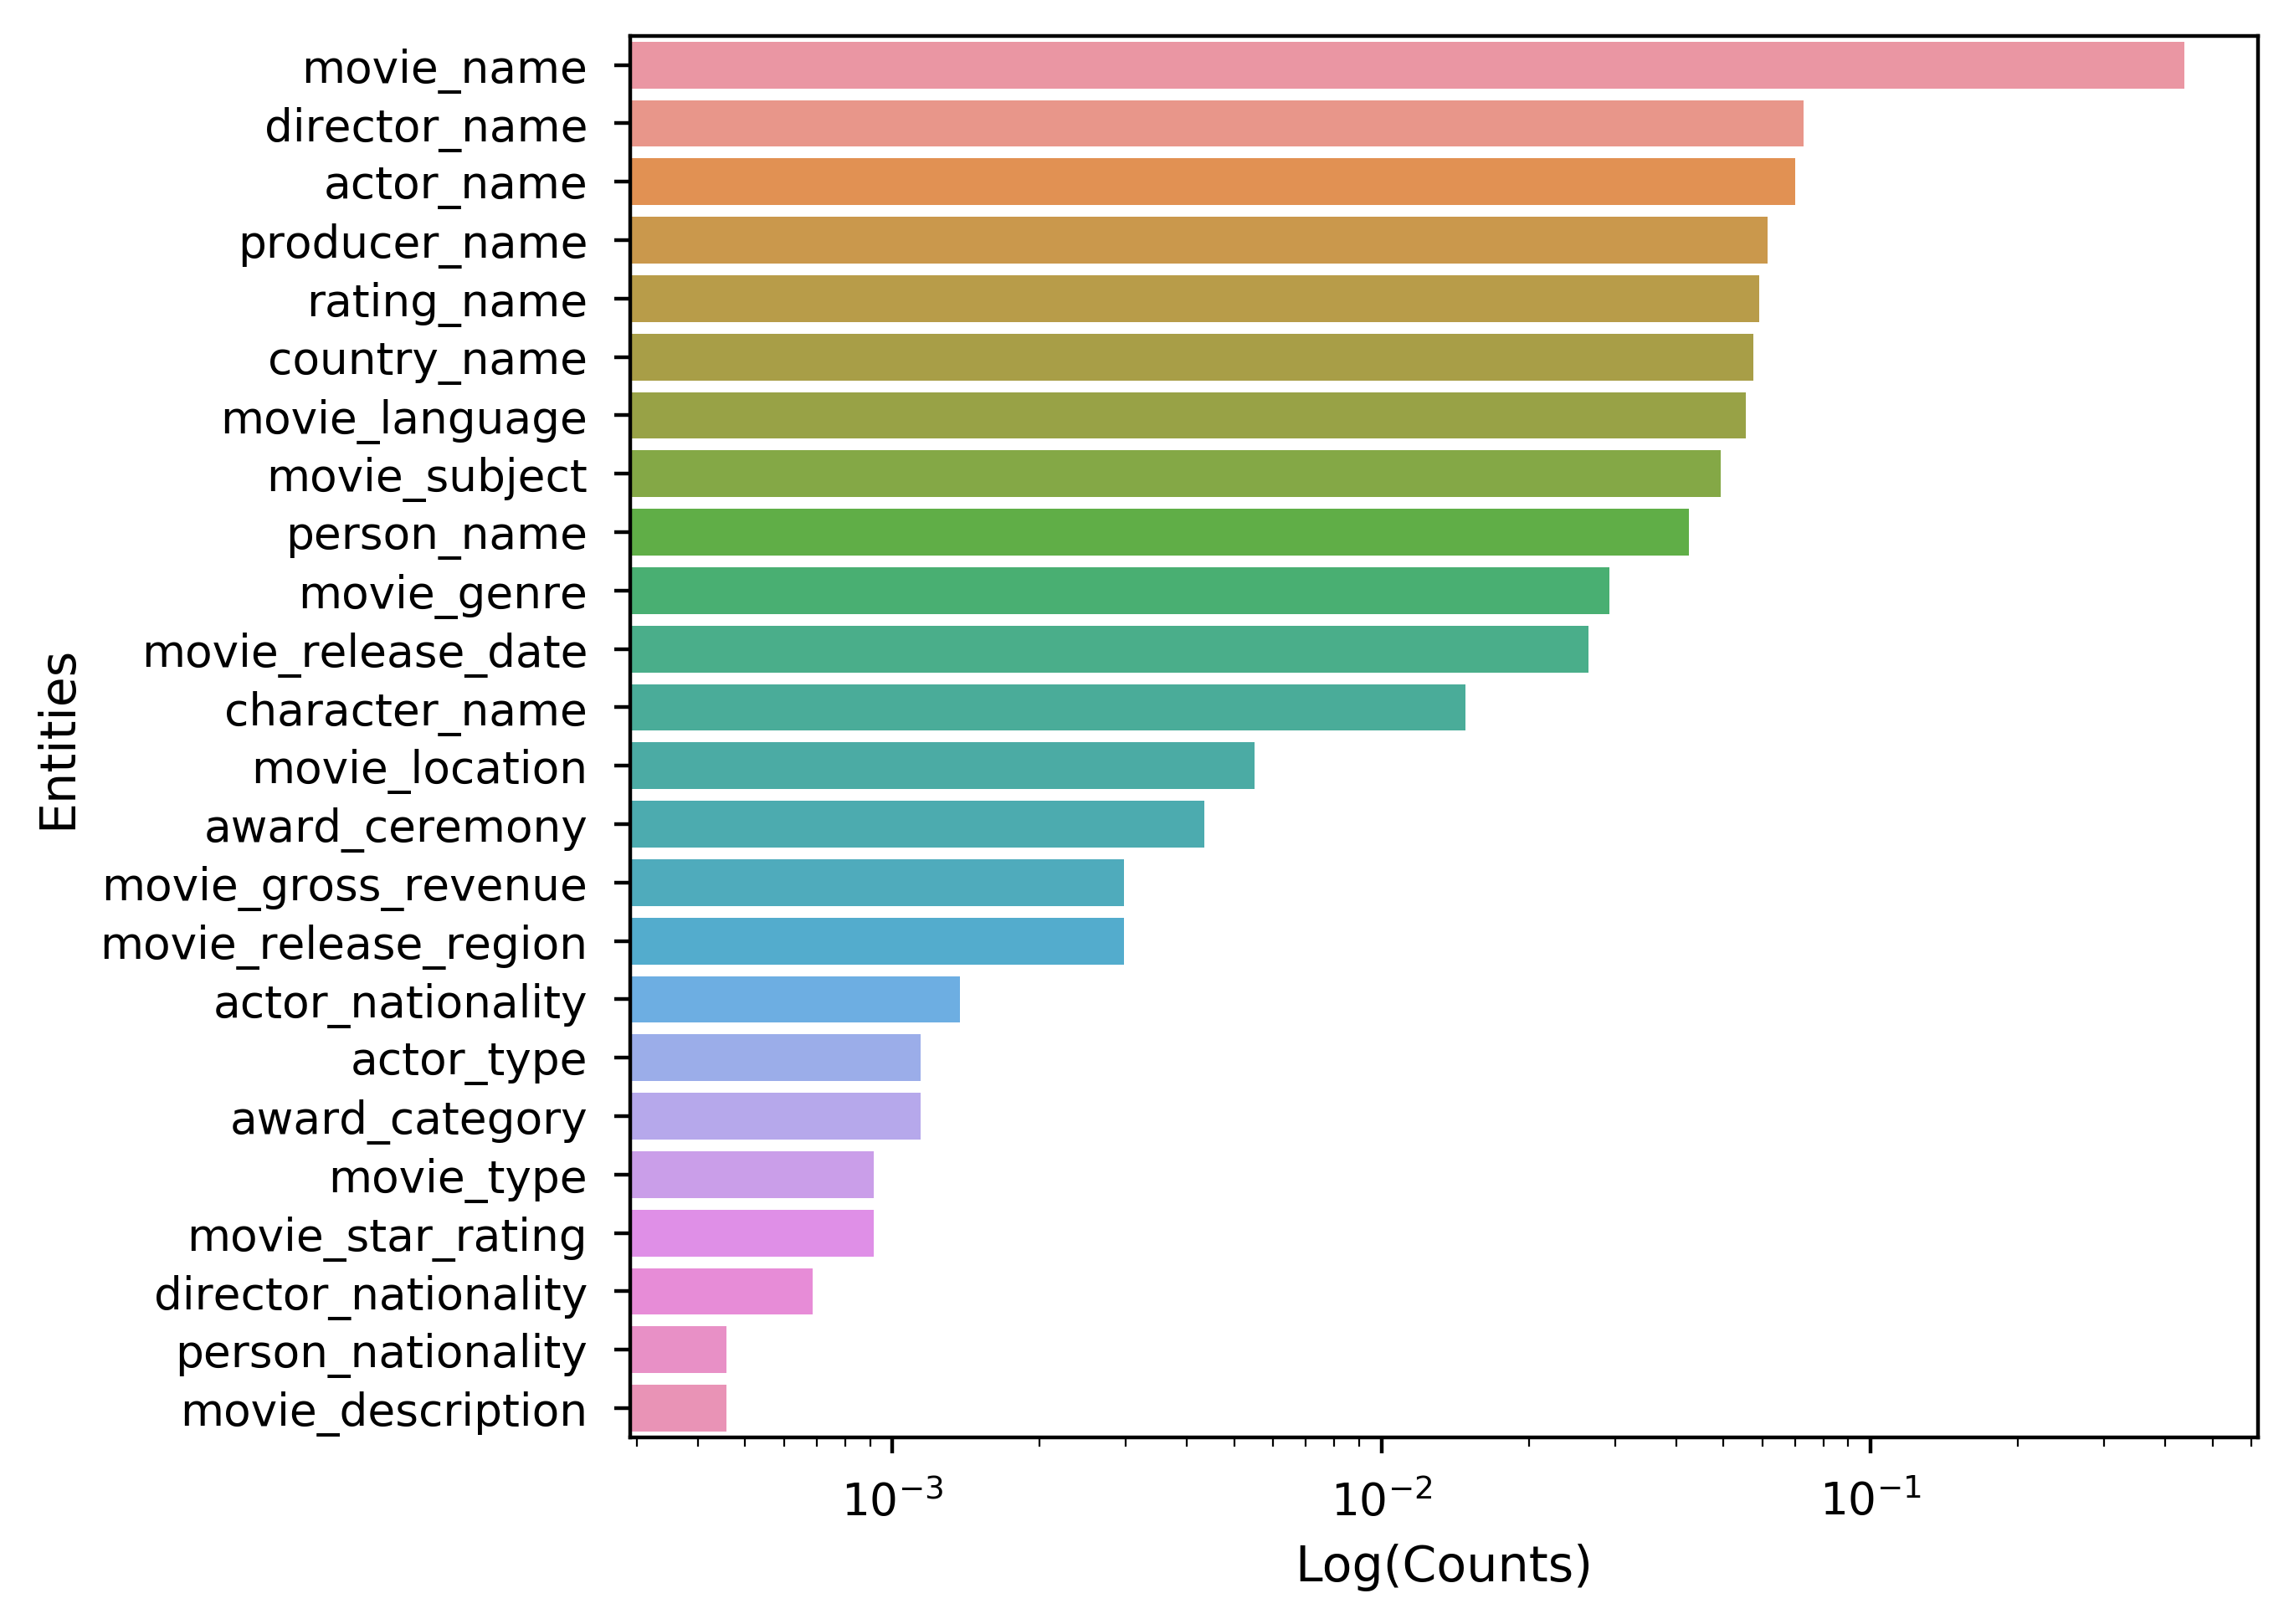
\includegraphics[scale=0.5]{entities_frequency}
		
		Here we can see that the \textit{movie name} entity is much more common than any of the other entities. But we do have a good amount of the entities we would expect our users to use the most, which is good so that the model is actually able to learn them.  
		
		Below is another graphic showing the count of intents (this has also been log scaled):
		
		\hspace*{-1.7cm}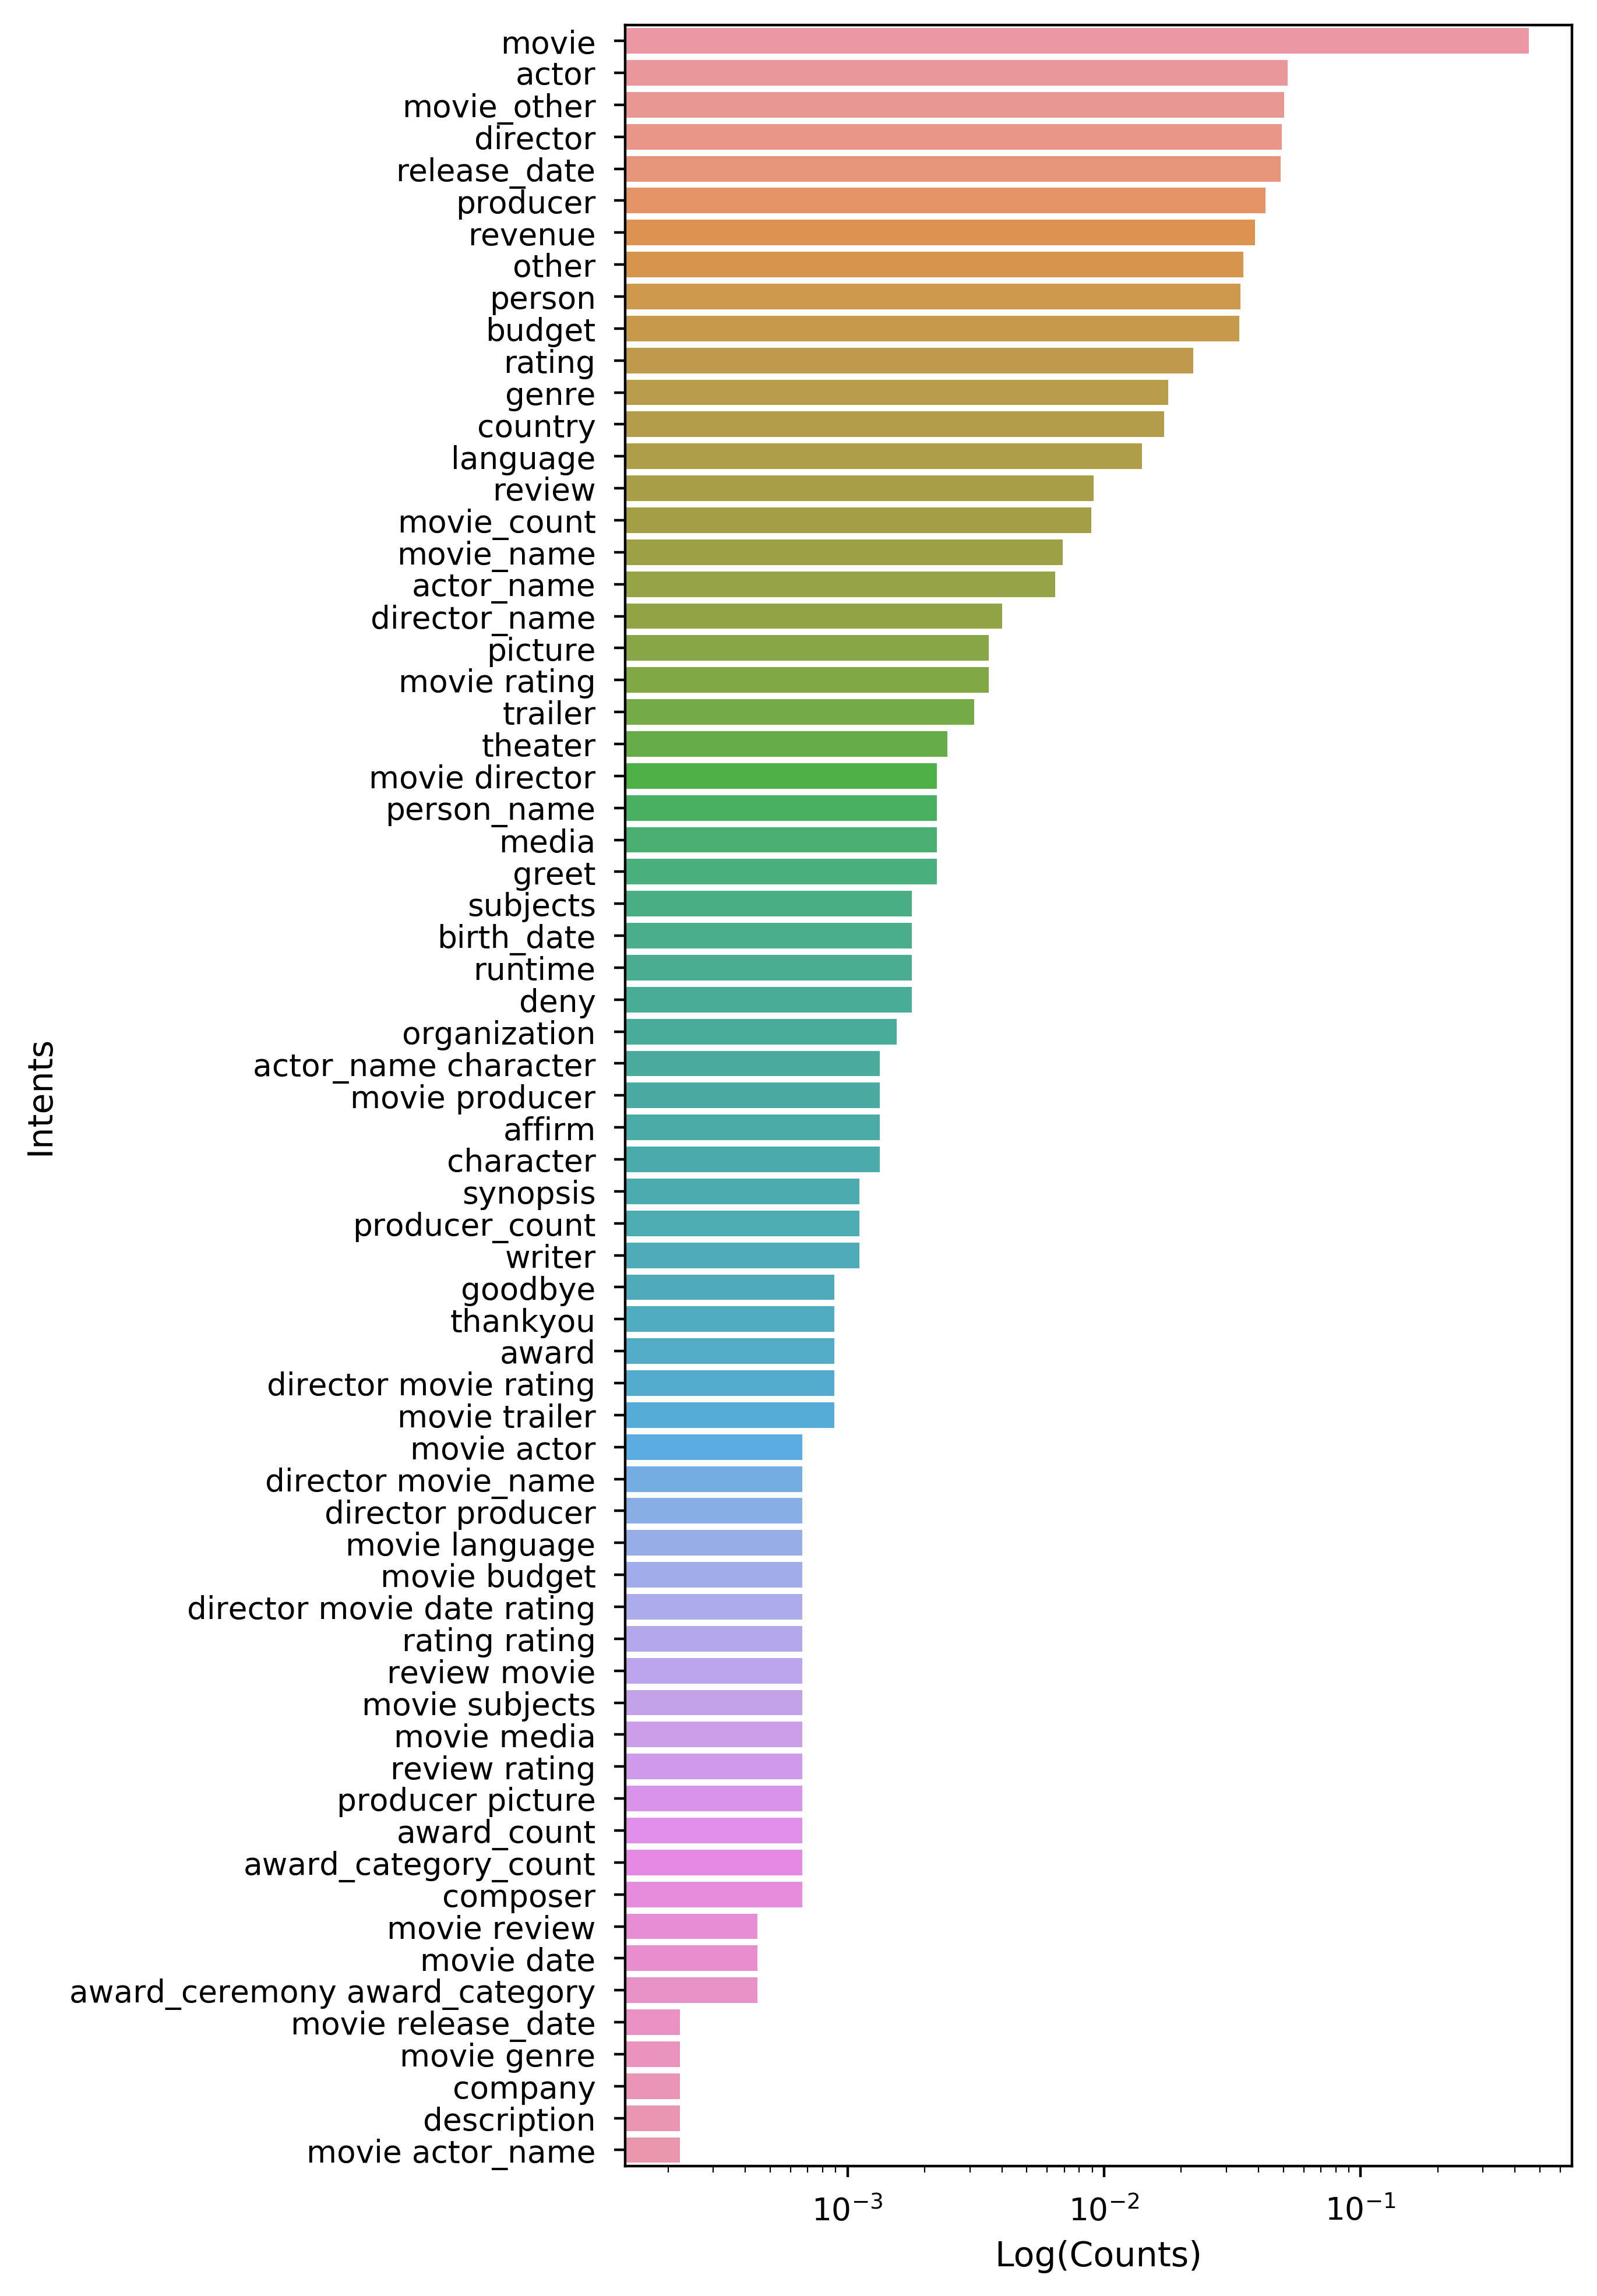
\includegraphics[scale=0.5]{intents_frequency}
		
		It is easy to note that also in this case \textit{movie} is the most common thing talked about. We can see that the difference between the most common item (\textit{movie}) and the least common one (\textit{movie actor name}) is much more pronounced for intents than it is for entities.
		
		Note that entity types may take many different values (for example, \textit{movie\_name} can be an entity representing diverse movie names in different sentences), while intents are always set (a sentence can only have one intent). This is the reason why we have fewer entities than intents.
		
	
	\subsection{Database}
	\label{ssec-database}
		
		The database basically contains all the knowledge that the bot has on the movie domain. If something is asked of the bot that is not in the database then it won't be able to answer. Each row in the database contains the following information for one movie:
		
		\begin{itemize}
		\setlength\itemsep{-0.48em}
			\item Title 
			\item Actors
			\item Director
			\item Genres
			\item Country where it was made
			\item Release date
			\item Original language
			\item Duration in minutes
			\item If it was released in color or not
			\item Budget
			\item Plot keywords
			\item Gross revenue
			\item IMDB score
			\item Likes on the movie's Facebook page
			\item Link to the movie's IMDB page
		\end{itemize}

		
		The original database was mainly fine, there were some empty columns but in those cases the bot will tell the user that it doesn't have the information to answer. However there was one issue that required to modify the database to fix it and it was that some rows had as \textit{release date} years that were not possible (ie: \textit{18000000}), so all of the publishing years above 2018 were deleted.


\section{Bot Modules}
\label{sec-bot-modules}

	The bot is composed of 2 main modules: the \textbf{NLU Module} and the \textbf{Dialogue Module}. These have quite different functionalities but work in conjunction to make the bot work correctly. Below is a brief explanation of each and their components.

	\subsection{NLU Module}
	\label{ssec-nlu-module}
	
		The NLU module is in charge of recognizing what are the \textit{intents} and \textit{entities} in a sentence. It can be thought of as the module that is in charge of translating what the user wants so that the bot's core functionality can understand it. 
		
		But before we can start talking about the NLU module we need to make some definitions:
		
		\begin{description}
			\item[entities] 
			entities are the pieces of text in a sentence that the NLU module identifies as \textit{relevant} and to which it assigns a name (ie, \textit{comedy} is labeled with the entity \textit{movie genre}). These are what we want the NLU module to extract from a sentence.
			
			\item[intents] 
			the intents are "\textit{the meaning behind a sentence}". They're the kind of things we expect the user to say and which we can handle (ie, \textit{show me comedy movies} has the intent of \textit{show movies}). 
		\end{description}
	
		The bot uses the knowledge on \textit{entities} and \textit{intents} provided by the NLU module to decide what to do next and how to do it.
		
		\subsubsection{Rasa NLU}
		\label{ssec-rasa-nlu}
			
			To create the NLU module, the \textbf{Rasa NLU} \cite{rasanlu} library was used. It provides most of the functionality out of the box, what we need to do is choose a \textit{pipeline} and provide it with the training examples so that it can train the models.
			
			The core idea behind Rasa NLU is that of a pipeline. The pipeline is composed of different components, and when a new message is given to the NLU module, it passes through each component of the pipeline in a sequential manner. The components in the pipeline are each in charge of doing different things. For this bot, the \textit{spacy\_sklearn} "standard" pipeline is  used, which is one that is already defined in the library itself. 
			
			According to \cite{rasanlu} the components (in the order of processing) of the \textit{spacy\_sklearn} pipeline are:
			
			\begin{description}
				\item[1. nlp\_spacy] 
				this component is in charge of initializing Spacy structures. It is the first component in the pipeline since all other components depend on it. Possible parameters that can be passed to this component are: 
				\begin{enumerate*}
					\item \textit{model} -- says which Spacy language model to load (ie: \textit{en}, \textit{de}, \textit{en\_core\_web\_md}, etc). The value used for this parameter is \textit{en}.
					\item \textit{case\_sensitive} -- when retrieving word vectors this parameters defines if word casing is relevant or not (in other words: if words with different casing should be considered as different words). The value used for this parameter is \textit{false}. 
				\end{enumerate*}
				
				\item[2. tokenizer\_spacy] 
				creates "tokens" from the words in the sentence by using the Spacy language model loaded in the previous step. It basically consists of segmenting the sentence into words, symbols and punctuations. More information on Spacy's functionality, including the tokenization process, can be found in \cite{spacy-tokenization}.
				
				\item[3. intent\_entity\_featurizer\_regex] 
				creates regex features by looking at the regular expressions defined in the training data (if any). These features will later be used by the \textit{ner\_crf} component for entity extraction and by \textit{intent\_classifier\_sklearn} for intent classification.
				
				\item[4. intent\_featurizer\_spacy] 
				creates features for intent classification using the spacy featurizer. It basically adds the spacy word vectors to the other text features (if any) of a sentence.
				
				\item[5. ner\_crf] 
				uses conditional random fields to extract entities. This component makes use of features created in previous components as well as features created by itself. The most likely set of tags is calculated and returned. Possible parameters that can be passed to this component are: 
				\begin{enumerate*}
					\item \textit{features} -- we can define features for the current, previous and next word. The features used for the previous and next words are: \textit{the lowercase representation of the word}, \textit{if the word is a title}, and \textit{if word is uppercase}. For the current word the used features are: \textit{the lowercase representation of the word}, \textit{the word 'bias'}, \textit{the last 2 and 5 characters}, \textit{the first 2, 3 and 5 characters}, \textit{if word is uppercase}, \textit{if the word is a title}, and finally \textit{if the word is a digit}.
					
					\item \textit{BILOU\_flag} -- if we want to use BILOU tagging or not. The value used for this parameter is \textit{true}.
					
					\item \textit{max\_iterations} -- It specifies the maximum number of iterations for the optimization algorithm. The used value is \textit{50}.
					
					\item \textit{L1\_c} -- Specifies the L1 regularization coefficient. The used value is \textit{0.1}.
					
					\item \textit{L2\_c} -- Specifies the L2 regularization coefficient. The used value is \textit{0.1}.
				\end{enumerate*}
				
				\item[6. ner\_synonyms] 	
				Maps synonymous entity values to the same value: If the training data contains defined synonyms then this component will ensure that the relevant detected entities are mapped to the same value.
				
				\item[7. intent\_classifier\_sklearn] 
				employs an SVM that uses features extracted in previous components so as to define what is the \textit{intent} of a sentence. The SVM employs a \textit{linear kernel} and the optimal value for the \textit{C} parameter is found by doing a grid search on the following values: \textit{1, 2, 5, 10, 20, 100}.
				
			\end{description}
			
			Some of these components, like the \textit{entity} and \textit{intent} extractors, need to be trained so they can do their job correctly. This is done in the \textit{training phase}, in which we provide the NLU module with data and it automatically trains each component of the pipeline on it.


	\subsection{Dialogue Module}
	\label{ssec-dialogue-module}
		
		The dialog module is the second main part of the bot, and can really be thought of as the logic behind the bot's actions. As said above, the NLU is in charge of translating what the user means into data that the bot can understand. The \textit{Dialogue Module} is the part that does this \textit{understanding}.
		
		
		\subsubsection{Rasa Core}
		\label{ssec-rasa-core}	
		
			To build the dialogue module, the \textbf{Rasa Core} \cite{rasacore} library was used. This provides lots of built-in functionality, we only need to specify what is needed for the bot to work as we want it to. Rasa Core will take care of integrating itself with the NLU module, remembering entities, training the dialogue policies (more on this later), and basically setting up a framework around which to build the bot's logic. 
			
			The main configuration file of the dialogue module is the \textit{domain file}, in this we specify the following information:
			
			\begin{description}
				\item[slots] these can be thought of as the "entities" we want the bot to "remember" when they're detected in a sentence.
				\item[entities] these are a list of all the entities we expect the NLU module to recognize.
				\item[intents] these are all the intents we expect the NLU module to recognize.
				\item[templates] these are simple, canned, phrases that our bot may utter as a response to a user's query.
				\item[actions] list of all the actions our bot is capable of doing. These may contain simple actions like uttering one of the \textit{templates} or, more complex, custom actions.
			\end{description}
			
			In the dialogue module we also define how the user interacts with the bot, specifically what are the \textit{channels of communication}. For our bot, the user can interact with it either via text (like a normal chat) or via voice. The implementation of the voice communication channel is discussed more in depth in section \ref{sec-speech}.
			
			Besides the domain file and the channel configuration, the dialogue module is also optionally composed of one or more \textit{Policies} and one or more \textit{Custom Actions}. For this bot, we've defined only one custom policy and some custom actions. 
			

		\subsubsection{Custom Actions}
		\label{ssec-custom-actions}	
			
			This bot makes use of some custom actions, specifically actions that handle answering questions on the movie domain. The list of custom actions and a brief description of each is the following:
			
			\begin{description}
				\item[ActionSearchPerson] 
				is in charge of searching for a person or persons (so, director/actor)
				
				\item[ActionSearchPersonInfo] 
				searches for information on a person, or gives the IMDB page of the person if no information is found in the database.
				
				\item[ActionSearchMovie] 
				searches for a movie given some criteria
				
				\item[ActionSearchMovieInfo] 
				searches for information on a movie(s) given some criteria. Or returns the movie's IMDB page link if the requested information is not in the database.
				
				\item[ActionAnswer] 
				shows the result of executing one of the previous actions to the user
				
				\item[ActionFalloutSlots] 
				implements a \textit{short term memory}. More on this in section \ref{ssec-forgetting}.
				
				
			\end{description}
			
			The action that gets executed at each turn is selected by the policy depending on what is the intent of the user in its last utterance. 

		\subsubsection{Policies}
		\label{ssec-policies}	
			
			The policies are one of the most important parts of a bot. They are what decide, given a user input already \textit{translated} by the NLU module, which action of the bot should be done next so as to handle the user's utterance in the best way possible. In a high-level view, policies receive a user utterance from the NLU module and return one probability for each possible action, which says how likely is it that the bot will execute said action next.
			
			For this bot, a conjunction or Rasa's own \textit{MemoizationPolicy} and \textit{KerasPolicy} together with a custom policy was used. Both the meimoization and keras policies are trained on a dataset of example conversations, in this way they learn to predict which is the action that should be done next. Both of these are used to handle "non-custom" actions (like greet, say goodbye, etc), while the custom policy is in charge of routing requests that need special treatment to the respective actions. 
			
			The custom policy takes in a request and the intent that the NLU module has assigned to it. If the intent is one that can be handled by one of the custom actions (ie, search for a movie, or information on a movie) then the corresponding action is selected as the one to be executed next. If the intent of the current request is not one that can be handled by the actions then this policy doesn't apport anything and lets the \textit{MemoizationPolicy} and \textit{KerasPolicy} decide what should be the next action.
			
			The KerasPolicy is an \textit{recurrent neural network} built with Keras \cite{keras}. The first layer is composed of an \textit{LSTM} with \textit{32} units followed by a \textit{fully connected} layer with a \textit{softmax} activation to actually get the probabilities of the possible actions. This model is given a list of the past actions and states, as well as the current state, to predict which should be the next action.
			
			The MemoizationPolicy remembers examples from the training data, if it encounters a situation that is the same as one in the training data then the next action chosen is the \textit{next} action we had in the respective training example. In our case we're limiting this \textit{remembering} to \textit{2} turns (this configuration is passed on to the the policy via the \textit{max\_history} parameter).
		
		
		\subsubsection{Forgetting}
		\label{ssec-forgetting}	
		
			This bot has a special action that doesn't really interact with the user, but is in charge of giving a \textit{short term memory} to the bot. As said before, the dialogue module has some \textit{slots} that are in charge of \textit{remembering} the respective entities when encountered in a user's utterance. Once they're encountered they're remembered until the end of the conversation. 
			
			This long-term memory mechanism may work fine for streamlined, goal oriented bots, where they have a clear goal (ie, make a restaurant reservation), and they need to get some information to accomplish it (ie, the kind of restaurant). The actions of getting this information to accomplish the end goal are the \textit{short term goals}, and the bot can simply switch from one to the other until it has all the information and can accomplish the end goal (ie, make the reservation). 
			
			However, our movie QA bot does not really live in a \textit{streamlined} environment. The strategy of remembering forever may work fine for short conversation with only one context (if the user only asks questions about one thing), but when it comes to longer conversations, or conversations with multiple unrelated contexts, then the bot will just end up with too much information in its memory (the slots) and won't be able to determine which of the information is actually relevant to the conversation and which isn't.
			
			The method used to counter this problem is that of replacing the \textit{persistent memory} with a \textit{short term one} in which slots have a lifetime and at each turn this lifetime is decreased by one, when the lifetime reaches 0 the slot is cleaned (the information it holds is deleted). If a user mentions information on an already existing slot then the lifetime of that slot is reset. Currently, each slot has a lifetime of 1 turn, meaning that it will be deleted at the end of the next turn (so, it may be used by the current and next turn's actions) if the slot is not \textit{renewed} by the user. The only exception is the slot that holds the \textit{movie name}, this is renewed if either the user mentions it explicitly or if a \textit{serch movie info} action is executed. 
			
			Note that the lifetime only gets reduced if the last executed action is one of our custom actions, so that if the bot does another action (like \textit{greeting}) or just doesn't understand what the users meant then the slot information is preserved for one extra turn. This ensures that the slot won't be cleaned prematurely.
			
			The lifetime ensures that the slots remain relevant for the current context. Once there is a context change and a slot is no longer relevant it gets cleaned. However, there is still the limitation that when the user is talking about something and then immediately asks something unrelated, the bot won't be able to notice the context change (although this also happens with the default, persistent memory approach). This context change problem happens unless the new context is on the same topic as the last one, meaning that the relevant slot will be updated with the new information.
			
		\subsubsection{Speech Channels}
		\label{sec-speech}
		
			The speech functionality was implemented by adding \textit{custom input and output channels} to the dialogue module. The used channels are basically variations of Rasa's default text I/O channels. 
			
			For the voice output channel, instead of only outputting the response to the console it is also given to a TTS service so that it will be spoken to the user. To add the TTS capability, the \textit{pyttsx3} \cite{ttspy} library was used.
			
			The input channel is slightly more complicated since we need to know when to start \textit{listening} for user utterances, and then we need to convert it to text. A basic interaction via the console was set up in which the user can specify he/she is ready to speak by pressing a key in the keyboard. After the user says its request, the audio is sent to an external speech recognition service, which then returns the text present in the audio. This text is then processed as a normal text input by the bot. The voice processing functionality was implemented by using the \textit{SpeechRecognition} \cite{SpeechRecognition} library.
			
			
\section{Evaluation}
\label{sec-evaluation}

	Here we evaluate the NLU module's performance when extracting \textit{entities} an \textit{intents}. It is not possible to actually evaluate the dialogue module since we're using a \textit{scripted policy} which works by routing certain intents to certain actions. This policy is fixed and non-trainable, so it makes no sense in evaluating the performance since it will always choose the expected action. 
	
	Remember that as we said in section \ref{ssec-rasa-nlu}, the NLU pipeline components in charge of extracting entities and intents are the \textit{ner\_crf} (using conditional random fields) and \textit{intent\_classifier\_sklearn} (using a linear SVM).
	
	Below are the result of evaluating the NLU module on a \textit{test set}:
	
	\begin{table}[h!]
		\centering
		\begin{tabular}{l|l|l}
			\textbf{Metric} & \textbf{Intent} & \textbf{Entity} \\ 
			\hline 
			F1-Score & 0.716 & 0.922 \\ 
			\hline 
			Precision & 0.707 & 0.921 \\ 
			\hline 
			Accuracy & 0.754 & 0.926\\ 
			\hline 
		\end{tabular} 
		\caption{NLU performance: \textit{intent} and \textit{entity} classification on test set}
		\label{table:1}
	\end{table}
		
	In table \ref{table:1} we can see that the performance of classifying entities is much better than that of classifying intents. This makes sense since there are much less entity than intent labels (\textit{\mnentitylabels} and \textit{\mnintentlabels} respectively).
	
	Below are the results of evaluating the NLU module via \textit{cross validation} on the whole dataset (training + test data). \textbf{5} folds were used to do the cross validation.
	
	\begin{table}[h!]
		\centering
		\begin{tabular}{l|l|l}
			\textbf{Metric} & \textbf{Train} & \textbf{Test} \\ 
			\hline 
			F1-Score & 0.930 & 0.765 \\ 
			\hline 
			Precision & 0.934 & 0.760\\ 
			\hline 
			Accuracy & 0.941 & 0.790 \\ 
			\hline 
		\end{tabular} 
		\caption{NLU performance: \textit{intent} classification cross validation}
		\label{table:2}
	\end{table}	
	
	We can see in table \ref{table:2} that the classification of training examples is quite good, and that of test examples is a bit better than it was when evaluating only on the test set. 
	
	Below is another table with the resulting performance of classifying entities via cross validation:
	
	\begin{table}[h!]
		\centering
		\begin{tabular}{l|l|l}
			\textbf{Metric} & \textbf{Train} & \textbf{Test} \\ 
			\hline 
			F1-Score & 0.962 & 0.930 \\ 
			\hline 
			Precision & 0.962 & 0.931 \\ 
			\hline 
			Accuracy & 0.964 & 0.934 \\ 
			\hline 
		\end{tabular} 
		\caption{NLU performance: \textit{entity} classification cross validation}
		\label{table:3}
	\end{table}	

	As expected, we see in table \ref{table:3} that both the performances when classifying entities from the training and testing examples are quite good. 
	

\section{Difficulties}
\label{sec-difficulties}

	This section mentions some of the difficulties encountered while developing and designing the bot.

	The main difficulty is how to know when a user has changed context. This is a notable problem, especially for open conversation (non-goal oriented) bots like this one. No solution was found but the \textit{short term memory} functionality provides a workaround.
	
	Another problem is when a query gets more than one result. Here we can suppose that the user is interested in all of the results or only on one of them. For this bot, when there are multiple results it was decided to display all of them to the user, in the most compact way possible.
	
	This takes us to the problem of how to know how much information is the user interested in. So, how much information is too much and how much is too little. We decided to provide more information when there was only one answer and less information when there were multiple ones.
	
	Another problem of a different nature was encountered when developing the voice input functionality: \textit{free} speech-to-text services (at least the ones tried during development) are not very good and it is quite common for them to return text that is not actually correct. This, in turn, may impact the \textit{perceived} performance of the bot. 
	
	Other questions that were not really answered are: How to differentiate between a question we don't support and one that was interpreted incorrectly. How to know when we need to ask for clarification when we don't have clear goals.


\section{Possible Improvements}
	
	The main possible improvement is that of joining similar \textit{intent} and \textit{entity} labels so as to reduce the number of different labels the NLU module has to predict. When looking at the entity and intent graphics in section \ref{ssec-nlu-data} it can easily be seen that many of them have similar names and possibly similar meanings. We could also remove the intents and entities that have very few examples (which means it is unlikely to find them in real life).
	
	Another possible change that might improve the performance is to the \textit{short term memory functionality}. Instead of thinking of the lifetime as \textit{turns} it can also be modeled with a probability of keeping the slot. This probability can decrease every turn. If set properly this might help to make it appear that the bot recognizes context changes. 
	
	A sure improvement of the voice input functionality would be to use a \textit{paid} speech to text service (or possibly a locally hosted one) so as to be able to properly recognize user input.

\section{Conclusion}
\label{sec-conclusion}
	
	The rasa stack provides a great framework for building chatbots. It already provides much of the functionality implemented by default, but is flexible enough so that we can make our bot behave as we want it to. 
	
	We've encountered one of the most common problems when building chatbots, that is, the problem of noticing when the context of the conversation has changed. This is especially problematic for bots like the one built here that have an \textit{open conversation} behavior (where they don't really have goals to accomplish). We've seen that making the bot forget information every turn makes it able to hold longer conversations without getting \textit{confused} on the context. This technique works well for the current bot where a user query depends at most on the previous 2 (since it's basically a QA system with context), but forgetting may not work so well for bots that don't have well defined goals and do need to have long-term memory (ie, a conversational bot that remembers information on the user's preferences). We suppose that a similar model, where we have long and short term slots, may work well as a possible solution. 
	


% include your own bib file like this:
\bibliographystyle{plain}
%\bibliography{acl2018}

%\bibliographystyle{plainnat}
\bibliography{bibliography}

%\bibliographystyle{acl_natbib}


\end{document}
